\documentclass[aspectratio=169]{beamer}

\mode<presentation>
{
  \usetheme{default}
  \usecolortheme{default}
  \usefonttheme{default}
  \setbeamertemplate{navigation symbols}{}
  \setbeamertemplate{caption}[numbered]
  \setbeamertemplate{footline}[frame number]  % or "page number"
  \setbeamercolor{frametitle}{fg=white}
  \setbeamercolor{footline}{fg=black}
} 

\usepackage[english]{babel}
\usepackage[utf8x]{inputenc}
\usepackage{tikz}
\usepackage{courier}
\usepackage{array}
\usepackage{bold-extra}
\usepackage{minted}
\usepackage[thicklines]{cancel}

\xdefinecolor{dianablue}{rgb}{0.18,0.24,0.31}
\xdefinecolor{darkblue}{rgb}{0.1,0.1,0.7}
\xdefinecolor{darkgreen}{rgb}{0,0.5,0}
\xdefinecolor{darkgrey}{rgb}{0.35,0.35,0.35}
\xdefinecolor{darkorange}{rgb}{0.8,0.5,0}
\xdefinecolor{darkred}{rgb}{0.7,0,0}
\definecolor{darkgreen}{rgb}{0,0.6,0}
\definecolor{mauve}{rgb}{0.58,0,0.82}

\title[2018-02-05-cmsoffline-oamap]{Data Analysis R\&D}
\author{Jim Pivarski}
\institute{Princeton University -- DIANA-HEP}
\date{February 5, 2018}

\begin{document}

\logo{\pgfputat{\pgfxy(0.11, 7.4)}{\pgfbox[right,base]{\tikz{\filldraw[fill=dianablue, draw=none] (0 cm, 0 cm) rectangle (50 cm, 1 cm);}\mbox{\hspace{-8 cm}
\includegraphics[height=1 cm]{princeton-logo-long.png}
\includegraphics[height=1 cm]{diana-hep-logo-long.png}}}}}

\begin{frame}
  \titlepage
\end{frame}

\logo{\pgfputat{\pgfxy(0.11, 7.4)}{\pgfbox[right,base]{\tikz{\filldraw[fill=dianablue, draw=none] (0 cm, 0 cm) rectangle (50 cm, 1 cm);}\mbox{\hspace{-8 cm}
\includegraphics[height=1 cm]{princeton-logo.png}
\includegraphics[height=1 cm]{diana-hep-logo.png}}}}}

% Uncomment these lines for an automatically generated outline.
%\begin{frame}{Outline}
%  \tableofcontents
%\end{frame}

% START START START START START START START START START START START START START

\begin{frame}{Tools for data analysis}
\vspace{0.5 cm}
\begin{block}{\underline{Eventual goal}}
\vspace{0.15 cm}
{\bf Query-based analysis:} let physicists do their analysis by querying a central dataset instead of downloading and managing private skims. Remove an expensive middleman!
\end{block}

\vspace{0.5 cm}
\begin{block}{\underline{Existence proof}}
\begin{enumerate}
\item I've worked with such systems at several large companies as a statistical consultant, regularly querying terabytes in seconds.
\item I accessed Google BigQuery to prepare part of this talk (2~TB in 30~sec).

Giant SQL servers are common in industry: this one is publicly accessible.
\end{enumerate}
\end{block}
\end{frame}

\begin{frame}{Google BigQuery}
\vspace{0.5 cm}
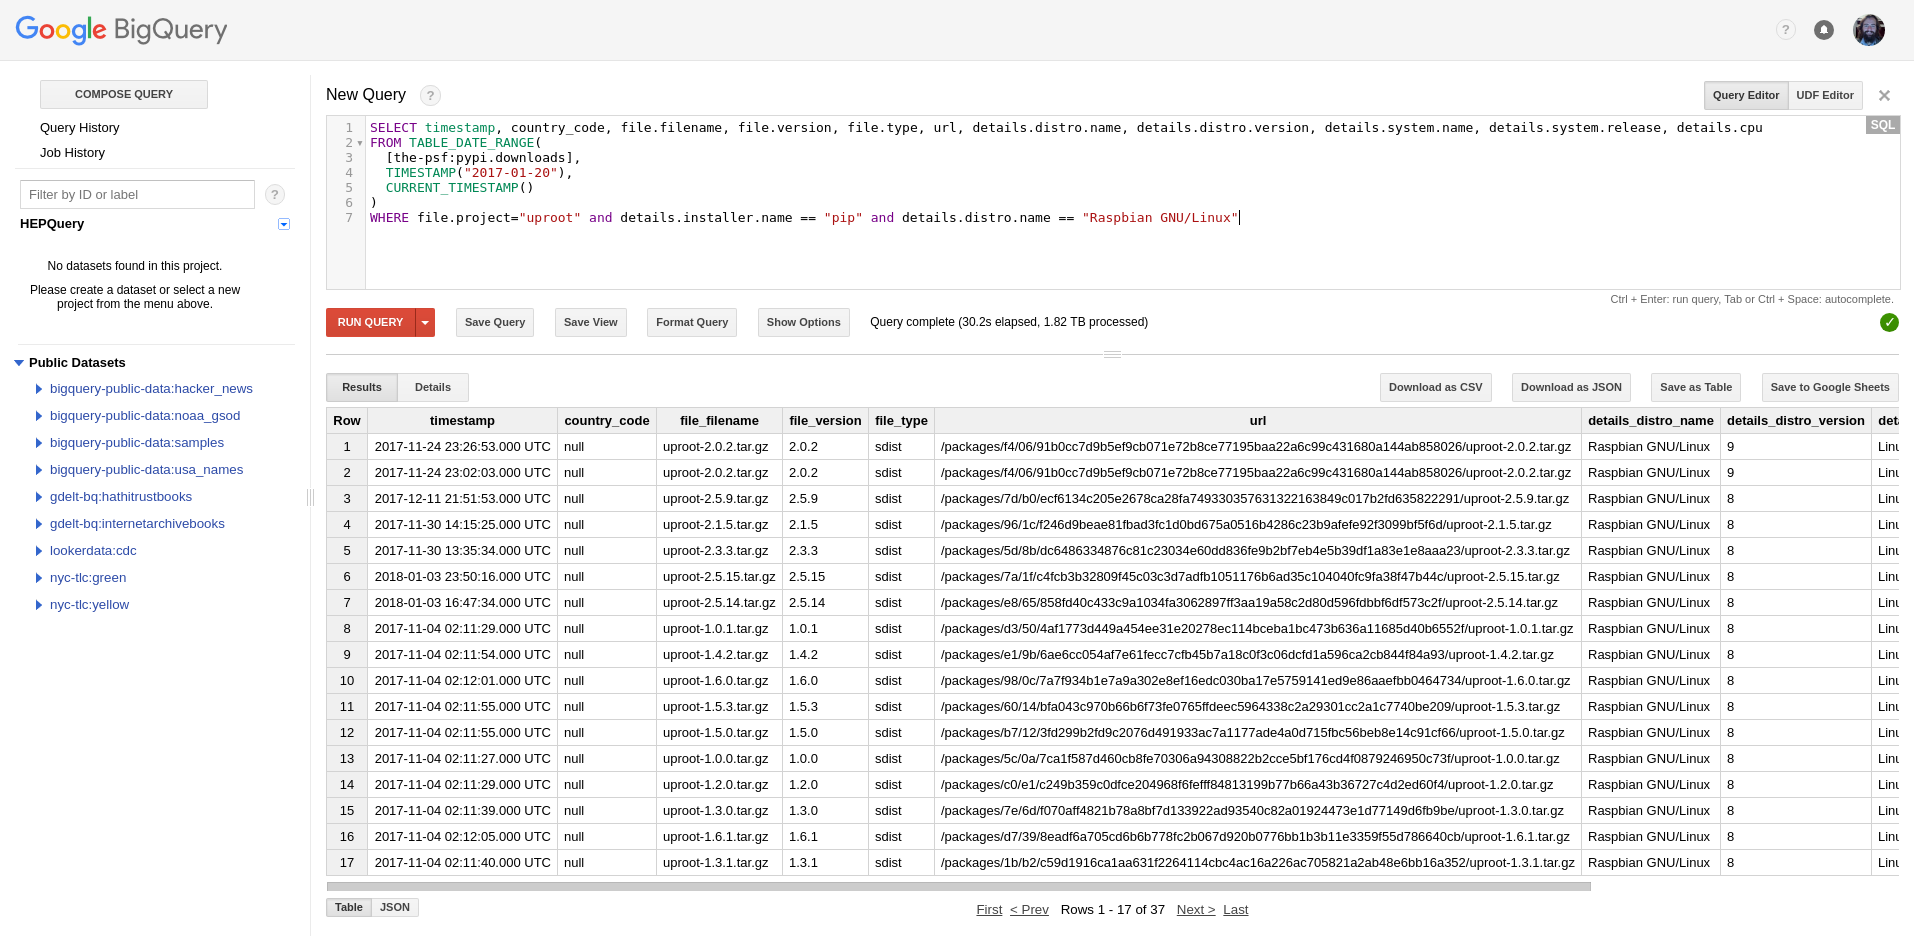
\includegraphics[width=\linewidth]{bigquery.png}
\end{frame}

\begin{frame}{Steps and differences}
\vspace{0.5 cm}
\mbox{\hspace{-0.55 cm}\textcolor{darkblue}{We can't directly use these systems in HEP without a few changes:}}

\renewcommand{\arraystretch}{1.5}

\vspace{0.25 cm}\mbox{\hspace{-0.7 cm}
\begin{tabular}{p{0.26\linewidth} p{0.2\linewidth} p{0.21\linewidth} p{0.3\linewidth}}
& Google & HEP & what I'm developing \\\hline
Source data format & \mbox{Parquet, ORC,} Avro, BSON, \ldots & ROOT & \mbox{{\bf uproot:} array-centric} ROOT reader \\
Query language & SQL & Python or C++ & {\bf oamap:} columnar objects \\
Distributed storage & GFS/HDFS & {\it similar} (Ceph?) & {\it starting now} \\
Distributed processing & Dremel/Drill & \mbox{{\it similar} (Dask?} Zookeeper?) & {\it future} \\
User interface & \mbox{web dashboard,} \mbox{Google Sheets,} REST queries & TDataFrame, \mbox{PyROOT, Jupyter}, SWAN, Spark & {\bf Histogrammar:} \mbox{functional histogramming,} {\bf Femtocode} {\it (future)\ldots} \\
\end{tabular}}
\end{frame}

\begin{frame}{}




\end{frame}



\end{document}
